\chapter{La genealogia}

    \paragraph{}
    Resultaria estrany realitzar un projecte que parla o tracta la genealogia en tots els seus apartats i no realitzar una petita introducció que exposi en què consisteix aquesta ciència.

    No representa un objectiu del projecte comprendre l’estat actual de la genealogia en el món contemporani, ni el de crear un dibuix detallat de quines lleis en regulen les seves activitats. No obstant això, sí que es creu que donar una petita visió general dels problemes i preguntes que aquesta ciència pretén abordar pot ajudar a lectors del projecte o futurs estudiants a comprendre millor les  limitacions i oportunitats d'aquest sector.

    \section{Què és la genealogia?}

    \paragraph{}
    La \gls{genealogia} (del grec:  \emph{'genea', 'generació'}; i, \emph{'logos', 'coneixement'}) és també coneguda pel nom d’història familiar. Aquesta ciència consisteix en l’estudi de les famílies, el seguiment dels seus llinatges, tant ascendents com descendents i l’estudi de la història de les persones.

    Els genealogistes, o persones dedicades a la genealogia, tant en l’àmbit privat com personal, utilitzen com a recurs d’investigació arxius històrics rics en dades. Exemples d'aquests recursos poden ser les partides de naixement, documents de defunció, registres d’emigració o altres documents informatius del mateix caire.  L'objectiu d'aquests documents és obtenir informació sobre una persona o família per així poder demostrar relacions de parentesc i llinatge o bé, fets empírics relatius a la vida d'un individu en concret.

    Un altre recurs que es veu cada cop més utilitzat és l'anàlisi genètic, mètode que té una rebuda, demanda i interès més elevat en l’àmbit personal, que no pas en el científic. La finalitat principal d'aquest mètode és la d'esbrinar relacions familiars passades i presents de l'individu a través de l'anàlisi dels seus gens.

    Els motius pels quals una persona pot estar interessada a endinsar-se en el món de la genealogia són diversos. Un exemple podria ser el desig de situar la seva família en un marc més ampli dins de la història o bé, el sentiment de responsabilitat de cara a preservar la història familiar per les futures generacions.

    Els aficionats a la genealogia, que la practiquen com a hobby, generalment investiguen la seva ascendència o la d’una persona propera. Per altra banda, els professionals, acostumen a encarregar-se de realitzar recerques genealògiques per tercers, estudiar i ensenyar mètodes de recerca o mantenir les seves pròpies bases de dades.

    Cal entendre que la genealogia no tracta només de recopilar informació sobre el moment històric en què una persona va néixer, viure o morir, sinó també el de recollir informació sobre l'estil de vida que aquella persona va portar, les seves biografies o quins van ser els esdeveniments i motivacions que van conduir i marcar la seva existència. En altres paraules, podríem dir que una part de les preguntes que la genealogia pretén respondre és la de com van viure o quin caràcter van mostrar els nostres avantpassats al viure durant el transcurs d'esdeveniments històrics, com per exemple, la segona guerra mundial.

    Voldríem tancar aquesta secció indicant que si l'interès per la genealogia, ha anat en augment en els últims temps, és en gran part gràcies a la digitalització de documents, fet que ha permès que genealogistes amateurs disposin d’un ventall d’eines molt superior al que van disposar els seus avantpassats i per tant, que les possibilitats de mantenir un arbre familiar o realitzar recerca genealògica quedin a l'abast de tothom.

    \section{El paper de la genealogia en el transcurs de la història}

    \paragraph{}
    Com s’ha comentat en l'apartat anterior, avui en dia la genealogia és una ciència que busca en gran mesura respondre preguntes de caràcter personal, no obstant això, aquest no va ser sempre el seu objectiu principal.

    Històricament, en les cultures occidentals, les persones estaven interessades a mantenir-se ben informades sobre la seva ascendència de cara a fer latents les seves connexions amb nobles i governants. Generalment, la intenció era protegir la seva situació privilegiada o escapar de la precarietat. En aquesta època, el terme genealogia compartia significat amb el d'\gls{heraldica}, terme usat avui en dia per la ciència que estudia els escuts d’armes. Així doncs, fins a finals del segle XIX, la genealogia deixava la seva marca en la història com a eina utilitzada principalment per aquells amb drets de poder o riquesa adquirits a través de l’herència.

    Aquest exemple, que bé ens podria semblar distant en el temps, no és l’única mostra dels impactes històrics relacionats amb aquesta ciència i com veurem a continuació, existeixen altres exemples molt més propers.

    No cal tornar gaires anys enredera per veure com durant l’època de l’alemanya nazi ser capaç de demostrar l’afiliació a la "raça suprema" era necessari per sobreviure o inclòs poder casar-se de forma legal. Per aquest motiu, no ens ha d’estranyar que avui en dia, Alemanya, segueixi sense fer públics la major part dels registres genealògics del segle XX, doncs els fets històrics han portat a percebre la història familiar com un atac, o amenaça, a la privacitat i seguretat de les persones. Les conseqüències d'aquesta època de la història són conegudes per tothom i un no pot evitar entreveure certes relacions amb el camp de la genealogia.

    Per situar un exemple que ens ocupi si pot ser encara més de ple, podem veure el valor de la memòria històrica i dels sentiments d’unió amb els nostres avantpassats arran de la gran quantitat de publicacions i missatges personals, recordant als seus avantpassats i als temps que els va tocar viure, en relació al vuitantè aniversari de l'esclat de la guerra civil espanyola. De fet, Catalunya és un altre clar exemple contemporani, conjuntament amb Alemanya, de com la memòria històrica pot ser present en la cultura, vida i sentiments de bona part d’una nació. Tant en l’àmbit personal, com col·lectiu.

    Així doncs, podem concloure que la genealogia, no tant com a ciència sinó com eina, va desenvolupar, desenvolupa i probablement, seguirà desenvolupant, un paper important en la història de la humanitat. No hem d’oblidar que els problemes racials segueixen molt presents en l'actualitat de les nostres societats, Estats Units, n'ha estat últimament un clar exemple, i que és la raça sinó una característica més de les nostres característiques de naixement, o en altres paraules, de les nostres dades genealògiques.

    \section{Les lleis reguladores}

    \paragraph{}
    Les seccions anteriors han introduït i descrit les ocupacions principals de la genealogia en els àmbits professional i amateur, així com el paper d'aquesta en la història. També s'ha esmentat que moltes de les dades amb les quals aquesta ciència interactua són de caràcter personal i per tant, sensibles a un ús impropi si no són regulades i protegides sota certes circumstàncies.

    És per aquest motiu que bona part de les dades públiques enregistrades per l’estat, sobretot aquelles que afecten a persones que encara són vives, es troben regulades sota un conjunt de lleis i legislacions. Aquestes lleis varien de nació en nació i per tant, no existeix un estàndard de quina informació és accessible pel domini públic, quina no i sota quines circumstàncies aquesta informació pot ser accedida.

    En el cas de l’estat espanyol són dues les principals lleis que regulen l’accés a les dades genealògiques. La \gls{LOPD} i la legislació consolidada: Llei 20/2011, del 21 de juliol del Registre Civil.

    El registre civil espanyol conté informació detallada d'una persona relacionada amb el seu naixement, relacions d’ascendència i descendència, nom i cognoms, emancipació, declaracions de concurs o suspensió de pagaments, nacionalitat, etcètera, etcètera.  Com podem veure, aquest registre conté tota mena d’informació sensible i al mateix temps, de gran valor de cara a estudis genealògics.

    Els habitants d'Espanya podem demanar accés a l'entrada d'una persona al registre civil mitjançant la presentació d'una sol·licitud digital, escrita o presencial. Per aconseguir aquesta informació caldrà proporcionar tan dades personals pròpies com el motiu pel qual es vol poder accedir a la partida en concret. Motius recurrents són l'estudi genealògic, gestions administratives o simplement la recaptació d'informació.

    Per altra banda, accedir al gruix de la informació no és fàcil i els genealogistes porten xocant amb portes tancades des de fa molts anys. Relacionat amb aquest aspecte, durant l'any 2011 es va aprovar una nova llei del Registre Civil que tenia com a objectiu racionalitzar l'estructura del registre i desjudicialitzar-lo. Aquesta llei havia d'entrar en vigor a partir del 2014, data que va ser posposada fins al juliol del 2015 i recentment ha tornat a ser ajornada fins al 30 de juny del 2017.

    La part que farà referència sobre si el nou registre contemplarà l'accés al públic de cara a la recerca genealògica encara està a l'aire, però sembla que hi ha certa esperança gràcies a la inclusió del següent apartat en l'article 80:

    \begin{displayquote}
        4. Amb caràcter excepcional i amb finalitats d'investigació familiar, històrica o científica, es podrà autoritzar l'accés a la informació registral en els termes que reglamentàriament s'estableixin.
    \end{displayquote}

    Així doncs, sembla que un futur no molt llunyà, aquesta informació podria passar a ser explotable en grans escala de cara a estudis familiars, històrics o científics. Això si, sempre respectant la \gls{LOPD}.

    \section{Els codis ètics en la genealogia}

    \paragraph{}
    El fet que els genealogistes tinguin accés i treballin amb informació pública, però simultàniament, personal, provoca que la professió es vegi envoltada de codis ètics que tractin de protegir la integritat d'aquesta, el sentiment de professionalitat i la moralitat d'aquells que interactuen amb les dades.

    Els codis morals giren al voltant de dos eixos. La protecció de la informació referent a les persones vives i les bones praxis de cara a la manipulació i tractament de les dades.

    El primer eix, tal com hem indicat, fa referència a protegir a aquelles persones que encara són vives. En concret, es tracta d'evitar, en la mesura que sigui possible, publicar informació de caràcter personal que poguí resultar compromesa per un individu en concret.

    El codi moral que hi ha en el rerefons és que a cap persona li agradaria trobar informació personal publicada al núvol, on tothom la pot accedir, pel simple fet que es tracta d'informació `pública'. Per tant, cal respectar la privacitat de les persones i no publicar fets o dades compromeses independentment de l'opinió personal del genealogista.

    Com ja s'ha mencionat amb anterioritat, la genealogia tracta en gran mesura d'estudiar els nostres avantpassats i la història de tots aquells que van existir abans que nosaltres, per tant, el xafardeig i la tafaneria no tenen cabuda dins dels codis ètics i morals de la professió.

    La segona branca ètica es correspon a un seguit de bones praxis de cara a la utilització d'informació genealògica. Tot i que no es tracta d'un manual oficial, la següent llista de `regles' serveix per descriure i fer-nos una idea amb un alt grau de fiabilitat, del que significa el concepte de bones praxis en aquesta ciència:

    \begin{itemize}
        \item El genealogista mantindrà les fonts de referència i les citarà quan utilitzi dades fetes públiques per un altre individual o col·lectiu.
        \item El genealogista no compartirà ni utilitzarà informació no contrastada o amb altes probabilitats de ser errònia.
        \item El genealogista transmetrà seguretat i confiança a aquells que facin ús dels seus serveis.
        \item El genealogista donarà suport a aquelles iniciatives que preservin els fitxers públics i l'accés a aquests.
        \item Es tractarà amb cordialitat i respecte al personal de les facilitats d'investigació.
        \item El genealogista ajudarà en la mesura que sigui possible als altres genealogistes i organitzacions dedicades a la genealogia.
        \item El genealogista compartirà els resultats dels seus estudis i investigacions.
        \item No està permesa la invenció ni exageració de la informació.
        \item El genealogista complirà amb les lleis en rigor dels conjunts de dades que utilitzarà en els seus estudis.
    \end{itemize}

    \section{El procés de recerca genealògica}

    \paragraph{}
    A tota persona que li interessi realitzar recerca genealògica sobre la seva pròpia família o la d'una persona propera, se li suggereix el següent procés com a mètode de treball.

    El procés de recerca es desenvolupa en cicles i cada cicle consta de cinc fases. A continuació es detallen una a una:

    \begin{enumerate}
        \item \textbf{Identificar el que es coneix:} Identificar i revisar tota la informació inicial que es coneix. Pel final de la fase s’haurien de tenir recopilats, ordenats i documentats tots els esdevenimentals relacionats amb la família o persona a estudiar disponibles.
        \item \textbf{Decidir que es vol aprendre:} L’objectiu d’aquesta fase és identificar sobre quin individu es vol obtenir informació, que es vol aprendre d’aquesta persona i si és possible el temps i llocs aproximats en els quals aquesta persona va viure.
        \item \textbf{Seleccionar els arxius a consultar:} Aquesta fase resulta la més complexa de tot el procés. L’objectiu, ordenar de més a menys útils les diferents fonts de dades a consultar i quins arxius resulten més interessants.
        \item \textbf{Obtenir i consultar els arxius:} Durant aquesta fase es consultaran les fonts de dades seleccionades a l’apartat anterior. Al final d’aquesta, hauríem de tenir anotat tot allò que s’ha descobert i còpies dels documents que suporten els descobriments, ja sigui en format de fotocòpies, notes o qualsevol altra mena de suport físic o digital.
        \item \textbf{Utilitzar la informació:} Finalment, en aquesta fase, tocarà avaluar la informació descoberta, transportar la nova informació als formularis adients, organitzar la informació i compartir els resultats. Un cop finalitzades totes aquestes tasques s'estarà preparat per tornar a iniciar la roda del procés i seguir així amb la recerca genealògica.
    \end{enumerate}

    \paragraph{}
    La figura~\ref{fig:researchProcess} mostra les cinc fases d'aquest procés cíclic.

    \begin{figure}[h]
            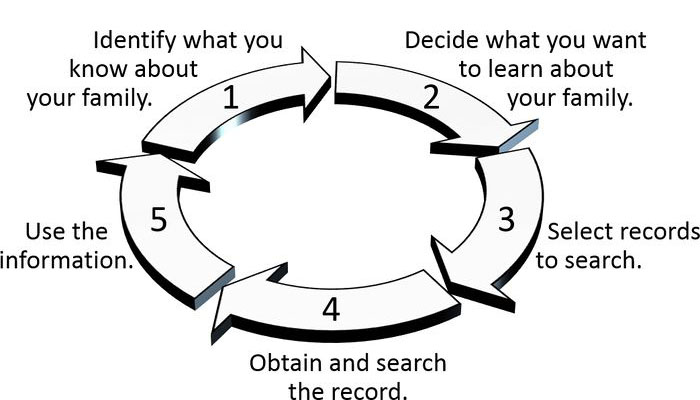
\includegraphics[scale=0.6]{02/researchProcess}
            \centering
            \caption{Procés de recerca genealògica.\label{fig:researchProcess}}
    \end{figure}

    \section{Conclusió}

    \paragraph{}
    Donem d'aquesta forma per conclosa la breu introducció a la genealogia. Com s'ha pogut observar, es tracta d'una ciència d'especial vocació personal, amb regulacions ambigües i rodejada de codis ètics i morals.

    Tot i les dificultats que tant genealogistes amateurs com professionals poden haver de fer front, aquesta ciència és capaç de desemmascarar i ajudar a comprendre les vivències dels nostres avantpassats i crear així un enllaç entre passat, present i futur. 

